\chapter{Описание и реализация нового алгоритма недоминирующей сортировки ENS-NDT-ONE}
\label{chapter3}

В данной главе опишем новый алгоритм ENS-NDT-ONE, который будет лучше подходить на роль одно из алгоритмов, на основе которых создается гибридный алгоритм. Так же в данной главе будет представлена и доказана асимптотическую оценку времени работы.

\section{Описание алгоритма}

Алгоритм ENS-NDT был изменен следующим образом: вместо множества деревьев теперь будем хранить одно дерево для всех точек, именно по этой причине, алгоритм назван ENS-NDT-ONE. Параметрами дерева, как в оригинальной версии алгоритма, будет размер корзины, ограничивающий максимальное количество точек, которое может содержаться в одной вершине, и вторым параметром будет глубина, начиная с которой размер корзины игнорируется, и точки перестают делиться на две при превышении первого порога. Так же как в оригинальном алгоритме дерево будет сбалансированным, это обеспечивается предварительно подсчитанной структурой $split$. На рисунке ~\ref{ndtree_new} представлено схематическое представление алгоритма ENS-NDT-ONE.

\begin{figure}[!h]
\begin{center}
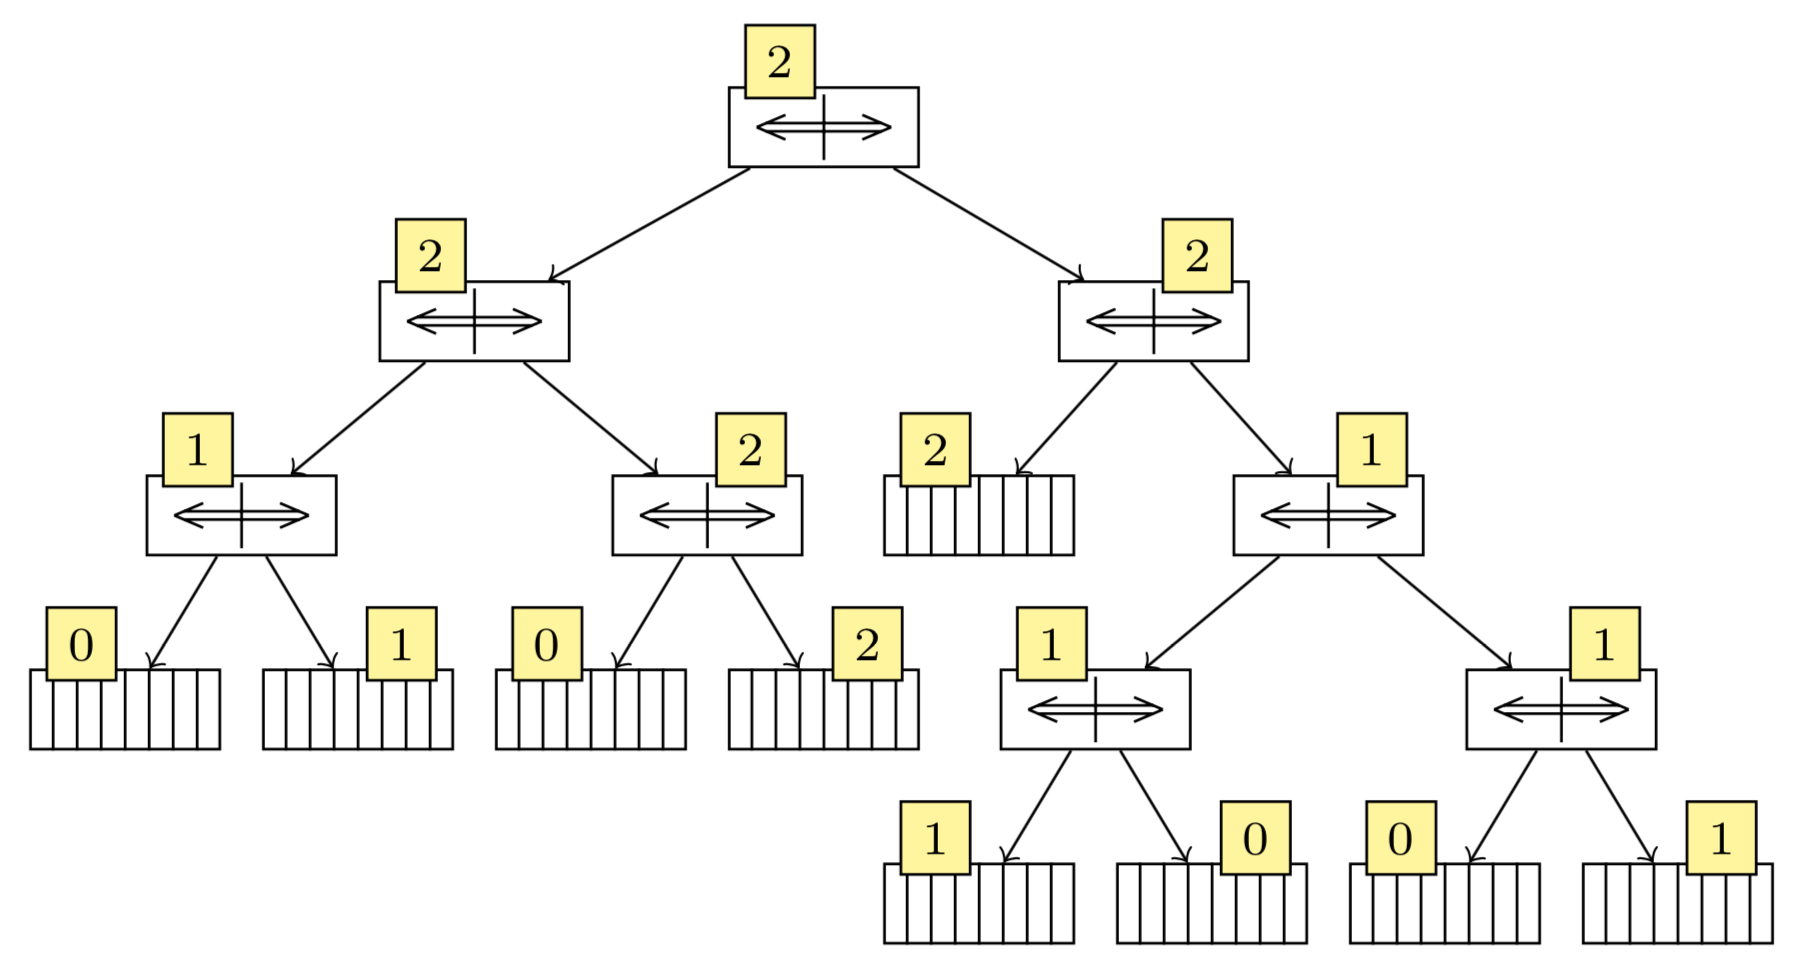
\includegraphics[width=15cm]{pic/ndtree_new.png}
\caption{Алгоритм ENS-NDT-ONE}.
\label{ndtree_new}
\end{center}
\end{figure}

Одним из преимуществ производительности алгоритма ENS-NDT было то, что, выполняя определение ранга для точки $p$ в некотором дереве, как только найденная точка доминирующая точку $p$, можно сразу же закрыть это дерево, так как больше точек из этого дерева не может влиять на ранг $p$. Это не так для алгоритма ENS-NDT-ONE, так как в дереве могут встретиться точки с большим или равным раном, чем ранг рассматриваемой точки $p$.

Чтобы предотвратить потери производительности, мы предлагаем хранить максимальный ранг всех точек на поддереве. Это позволит при определении точки с изначальным рангом $k$, не спускаться в поддерево с рангом $\leq k$. На фазе добавления точки в дерево необходимо не забыть обновить значения максимального ранга по пути добавления.

Адаптация для функции $HeplerA$ не требуется, так как это обычная недоминирующая сортировка. При обновлении ранга надо только учитывать предварительный ранг точки, и обновлять ранг только в том случае, если он был меньше, чем новый ранг. Напомним, что процедура $HeplerB$ принимает в качестве аргументов два множества, одно с окончательными рангами $L$, другое предварительными рангами $R$. В процедуре $HeplerB$ происходит обновление рангов множества $R$, по рангам множества $L$. Опишем работу алгоритма ENS-NDT-ONE с двумя множествами $L$ и $R$: 
\begin{enumerate}
  \item Обходим точки в лексикографическом порядке, как в оригинальном алгоритме.
  \begin{enumerate}
      \item Если точка принадлежит множеству с окончательными рангами $L$, добавляем точку в дерево с текущим рангом.
      \item Если точка принадлежит множеству с предварительными рангами $R$, то мы обновляем ранг рассматриваемой точки по дереву и не добавляем ее в структуру, так как ранжирование происходить только на основе точек из множества $L$.
  \end{enumerate}
\end{enumerate}

\section{Асимптотика времени работы}

Вероятность пропуска поддеревьев сильно влияет на производительность алгоритма ENS-NDT-ONE. В частности, для многих видов входных точек можно показать постоянную верхнюю границу $\alpha$ на вероятность входа в дочерний узел, который соответствует более высокому значению по критерию, рассматриваемому на данном слое. Из этого получаем верхнюю границу $O(MN^{\log_2(1+\alpha)})$ на один запрос и $O(MN^{1+\log_2(1+\alpha)})$ для всей сортировки, что строго быстрее, чем $\Theta(N^2M)$, когда $\alpha<1$. В худшем случае алгоритм ENS-NDT-ONE работает за $O(MN^2)$, однако зачастую время работы алгоритма сильно лучше. Например, на случайно сгенерированных точках в гиперкубе $[0; 1]^M$, $O(N)$ точек с вероятностью не более $1/2$ необходимо заходить в обоих детей в каждой не листовой вершине дерева. Таким образом получаем, что верхняя граница асимптотики времени работы равна $O(MN^{1+\log_2(1+1/2)}) \approx O(MN^{1.585})$.


\section{Реализация алгоритма ENS-NDT-ONE}

В данном разделе будет описана реализация алгоритма ENS-NDT-ONE. 

Вдохновившись идеями алгоритма ENS-NDT, был создан алгоритм ENS-NDT-ONE. Основным изменением алгоритма ENS-NDT стало то, что вместо множества деревьев для каждого ранга, теперь в структуре одно дерево. На листинге ~\ref{procedure_end_ndt_one} приведен псевдокод основного метода этого алгоритма, который принимает в качестве аргументов множество точек $P$, $M$ {---} размерность и $B$ {---} порог, максимальное количество точек в вершине. Для получения $split$ структуры используется функция $CreateSplits$, о которой можно почитать в первой главе данной работы.

Помимо этого, для ускорения процесса определения ранга, будем хранить максимальный ранг на поддереве, что позволит добавить следующую эвристику: если у поддерева максимальный ранг меньше ранга рассматриваемой точки, то это поддерево никак не может повлиять на ранг данной точки. 

\begin{algorithm}
\begin{algorithmic}[1]
\Procedure{ENS-NDT-ONE}{P, M, B}
    \State{$P \gets Sort(P, a^M \prec b^M, ..., a^1 \prec b^1)$}
    \State{$S \gets CreateSplits(P, M-1,B)$}
    \State{$\mathcal{F} \gets \{\{P_1\}\}$}
    \State{$\mathcal{T} \gets new NDTreeOne(S, B)$}
    \State{$InsertIntoNDTreeOne(\mathcal{T}, P_1)$}
    \State{$j \gets 1$}
    \For{$i = 2, ..., |P|$}
        \If{$P_{i-1} \neq P_{i}$}
            \State {$j \gets FindRankInNDTreeOne(\mathcal{T}, P_i)$}
            \State{$InsertIntoNDTreeOne(\mathcal{T}, \mathcal{P}_i)$}
        \EndIf
        \State{$\mathcal{F}_j \gets \mathcal{F}_j \cup {P_i}$}
    \EndFor
    \State{\Return {$\mathcal{F}$}}
\EndProcedure
\end{algorithmic}
\caption{Главная процедура алгоритма ENS-NDT-ONE.}
\label{procedure_end_ndt_one}
\end{algorithm}

В функцию $FindRankInNDTreeOne$ будет добавлен дополнительный аргумент, ранг точки $P_i$, тогда функция $FindRankInNDTreeOne$ в терминальной вершине будет иметь реализацию представленную на листинге ~\ref{procedure_find_rank_term}. А в нетерминальной вершине реализация представляет из себя два рекурсивных вызова на вершинах-потомках с одним только отсечением, если координата рассматриваемой вершины больше либо равна медианному значению, то в левого ребенка можно не заходить, то есть в поддерево, где по текущей координате все точки больше рассматриваемой, не найдется ни одной точки, которая бы доминировала нашу, следовательно заходить в такое поддерево нет смысла. На листинге ~\ref{procedure_find_rank_n_term} представлен псевдокод определения ранга в нетерминальной вершине.

\begin{algorithm}
\begin{algorithmic}[1]
\Procedure{FindRankInNDTreeOne}{$\mathcal{T}, p, r$}
    \If {$ maxRank < r$}
        \State {\Return {r}}
    \EndIf

    \If{$p[\mathcal{T}.splitCoordinate] >= \mathcal{T}.splitValue$}
        \State {$r \gets FindRankInNDTreeOne(\mathcal{T}.worseNode, P_i, r)$}     
    \EndIf
    \State {$r \gets FindRankInNDTreeOne(\mathcal{T}.betterNode, P_i, r)$}     
    
    \State{\Return {$r$}}
\EndProcedure
\end{algorithmic}
\caption{Процедура поиска ранга точки с предварительным рангом в нетерминальной вершине.}
\label{procedure_find_rank_n_term}
\end{algorithm}

\begin{algorithm}
\begin{algorithmic}[1]
\Procedure{FindRankInNDTreeOne}{$\mathcal{T}, p, r$}
    \If {$maxRank < r$}
        \State {\Return {r}}
    \EndIf
    \For{$i = |\mathcal{T}.points|, ..., 1$}
        \If {$\mathcal{T}.points[i] \prec p$}
            \State {\Return {$\mathcal{T}.ranks[i] + 1$}}
        \EndIf
    \EndFor
    \State{\Return {$r$}}
\EndProcedure
\end{algorithmic}
\caption{Процедура поиска ранга точки с предварительным рангом в терминальной вершине.}
\label{procedure_find_rank_term}
\end{algorithm}

Важно отметить, что если ранг на поддереве $< r$, то есть ранга рассматриваемой точки, то текущее поддерево не может повлиять на ранг точки, для которой происходит обновления ранга. В таком случае в строке 3 листингов ~\ref{procedure_find_rank_term} и ~\ref{procedure_find_rank_n_term} происходит выход из процедур.





